\documentclass[tikz,border=2mm]{standalone}
\usepackage{tikz}
\usetikzlibrary{arrows.meta,decorations.markings}

\begin{document}
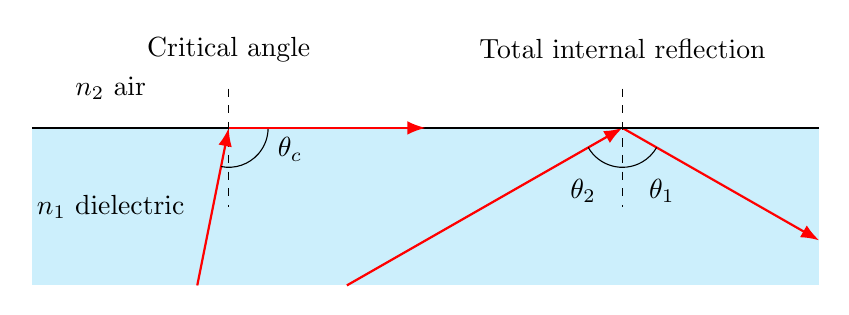
\begin{tikzpicture}[>=Latex, scale=1]


  \fill[cyan!20] (-5,0) rectangle (5,-2);

  \draw[dashed] (-2.5,0.5) -- (-2.5,-1);
  \draw[dashed] (2.5,0.5) -- (2.5,-1);


  \draw[red, thick, ->] (-2.9,-2) -- (-2.5,0);




  \draw[red, thick, ->] (-1,-2) -- (2.5,0);
  \draw[red, thick, ->] (2.5,0) -- (5,-1.4285714285714);



  \node at (-4, 0.5) {$n_2\ {\mathrm{air}}$};
  \node at (-4, -1.0) {$n_1\ {\mathrm{dielectric}}$};

  \node at (-2.5, 1.0) {Critical angle};
  \node at (2.5, 1.0) {Total internal reflection};




  \draw (-2.5,0) ++(258.69900676:0.5) arc (258.69900676:360:0.5)   node[below right] {$\theta_c$};
  \draw (2.5,0) ++(209.74488:0.5) arc (209.74488:330.25511:0.5) ;

  \node at (3, -0.8) {$\theta_1$};
  \node at (2, -0.8) {$\theta_2$};


  \draw[thick] (-5,0) -- (5,0);
  \draw[red, thick, ->] (-2.5,0) -- (0,0);


\end{tikzpicture}
\end{document}